\documentclass[11pt,a4paper]{article}
\usepackage[utf8]{inputenc}
\usepackage[spanish]{babel}
\usepackage{url}
\usepackage{hyperref}
\usepackage[margin=1.5cm]{geometry} % Reducción de márgenes
\usepackage{enumitem} % Para ajustar espaciado en listas
\usepackage{graphicx} % Para incluir imágenes

% Ajuste a interlineado
\renewcommand{\baselinestretch}{0.95}

\title{\textbf{Tarea 1: Herramientas para Alineamiento de Frecuencias en Bioinformática}}
\author{José Benavente}
\date{}

\begin{document}
	
	\maketitle
	
	\section*{Needleman-Wunsch Global Alignment App}
	\noindent Esta herramienta (\url{https://bgmp.github.io/bimm143_W20/class-material/nw/}) implementa el algoritmo clásico de programación dinámica para alineamiento global de secuencias.
	
	\noindent \textbf{Características:} 
	\begin{itemize}[noitemsep,topsep=0pt,leftmargin=*]
		\item Interfaz interactiva que muestra la construcción de la matriz paso a paso
		\item Personalización de puntajes para Match, Mismatch y GAP
		\item Visualización del camino de retroceso (traceback) para el alineamiento óptimo
	\end{itemize}
	
	\noindent \textbf{Aplicaciones:} Ideal para estudiantes y educadores que buscan comprender visualmente el funcionamiento del algoritmo. Facilita el aprendizaje de conceptos fundamentales de programación dinámica en alineamiento de secuencias.
	
	\begin{figure}[h]
		\centering
		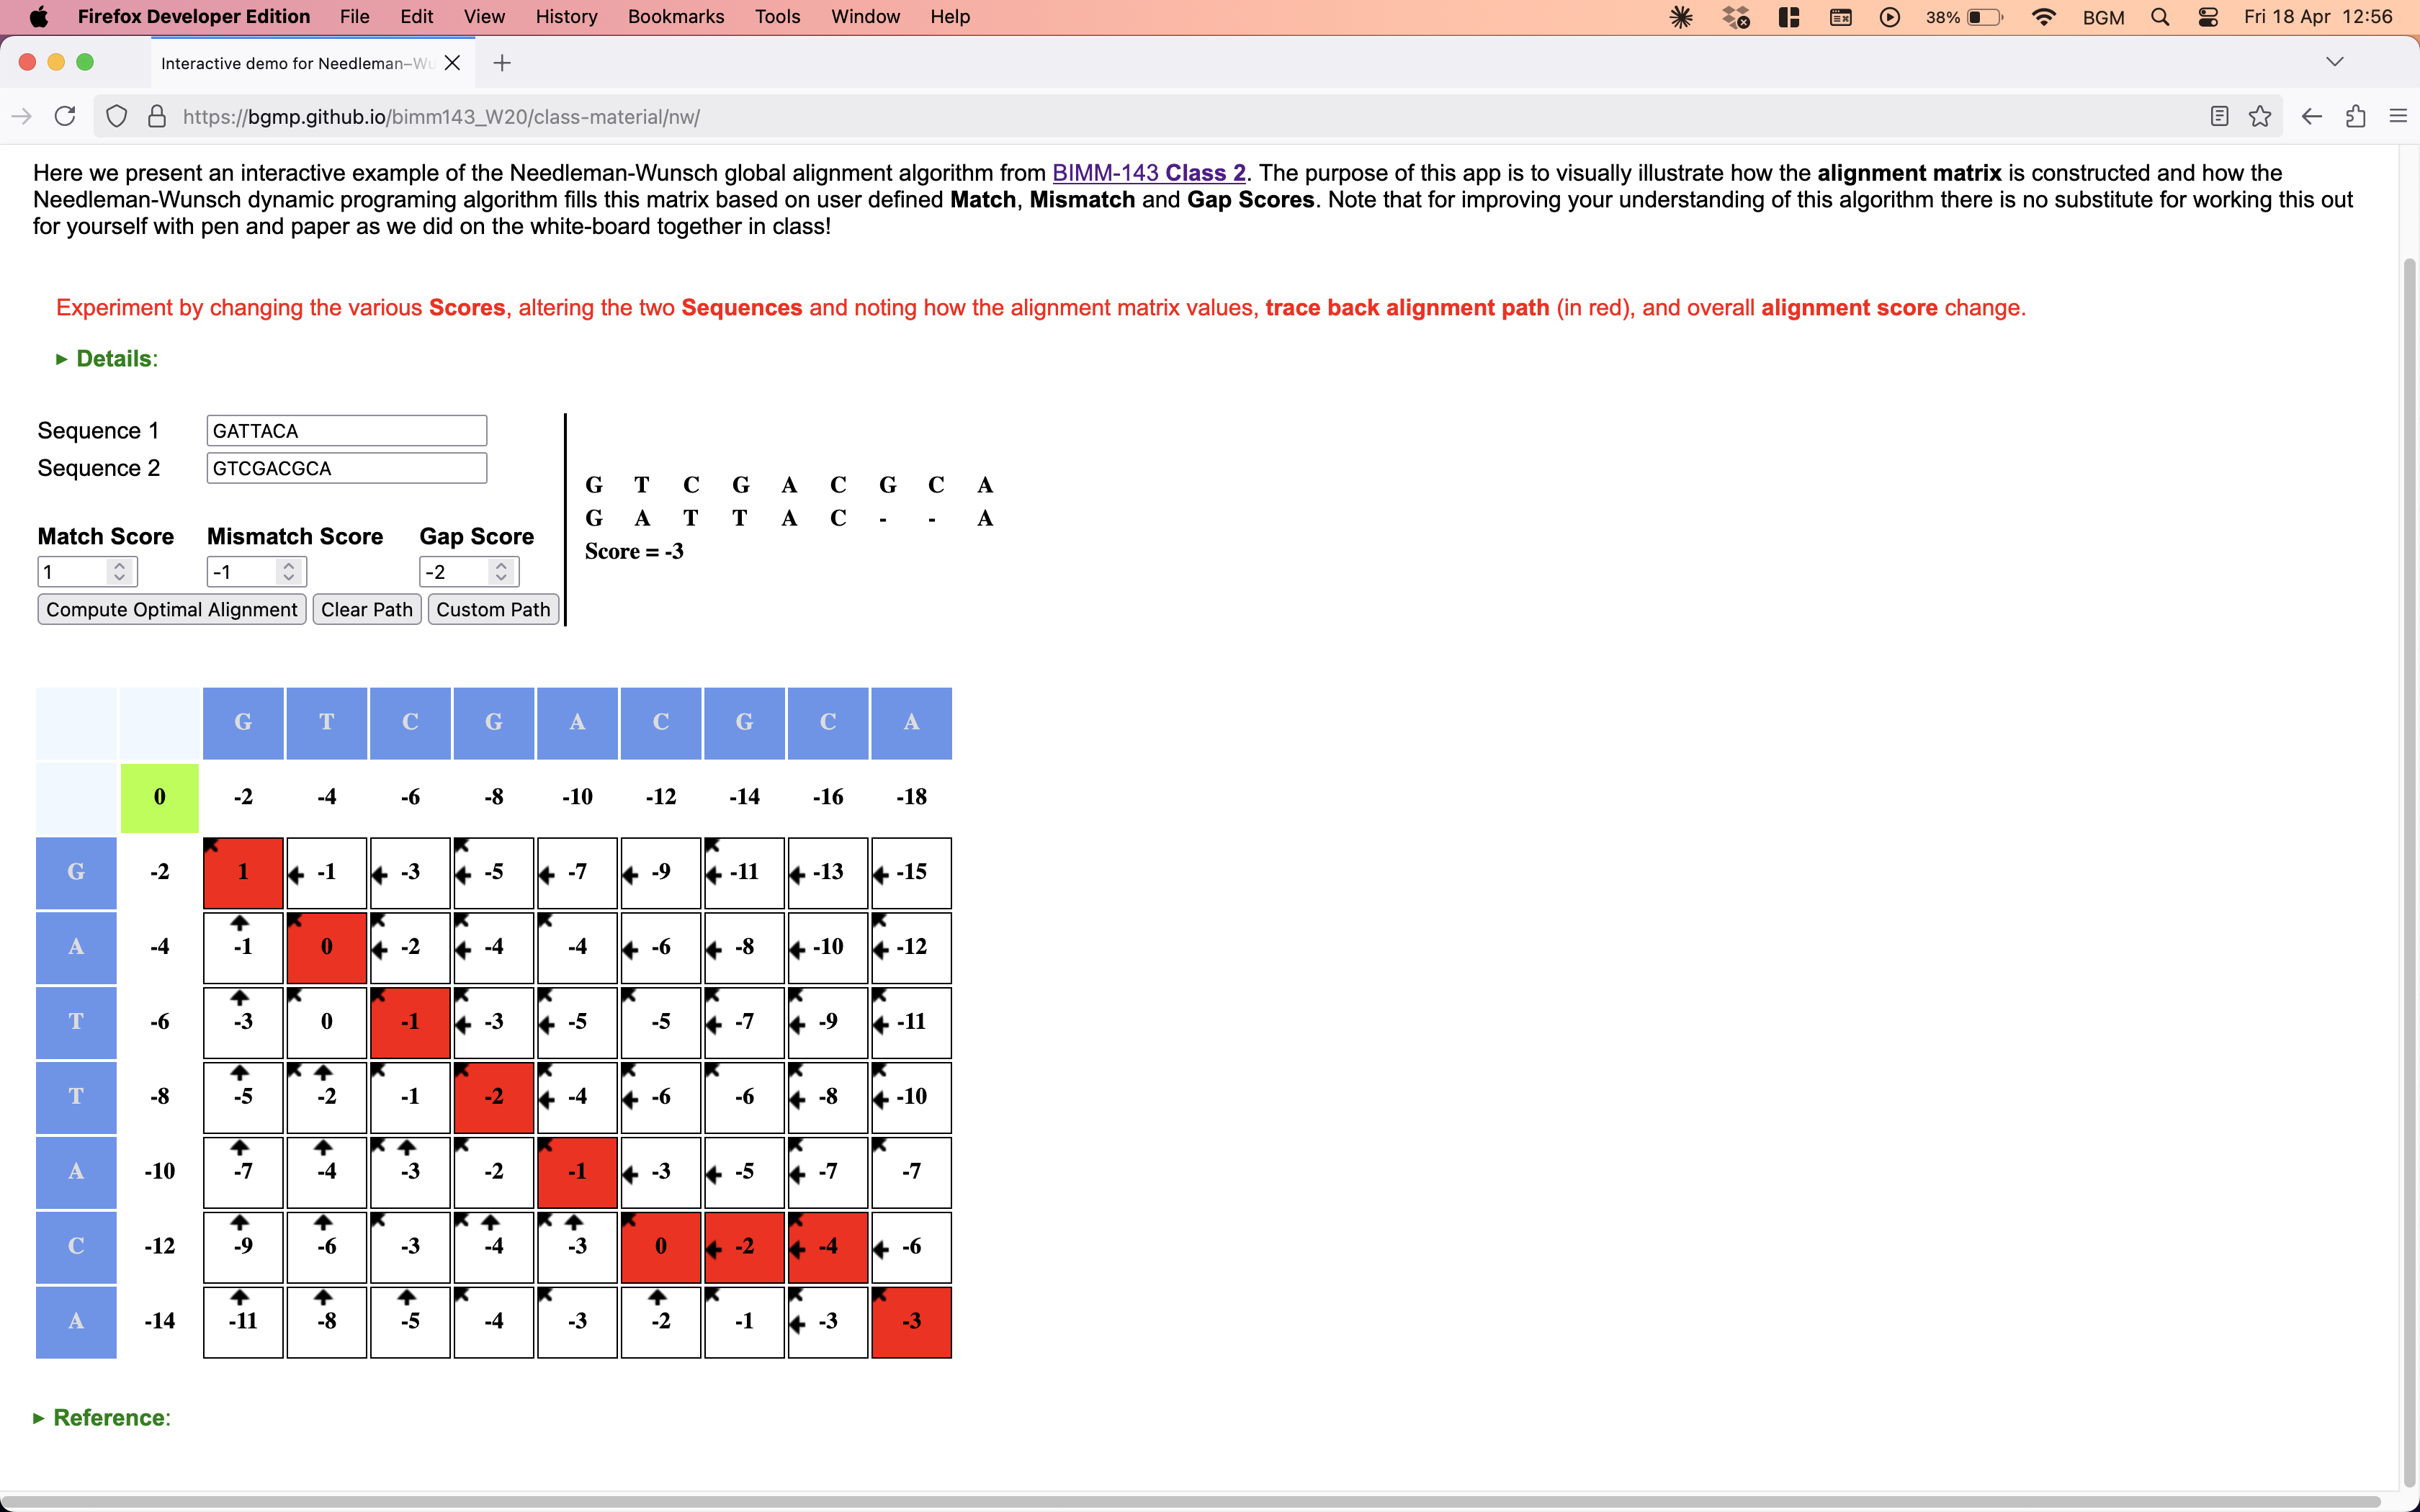
\includegraphics[width=0.7\textwidth]{img/needleman.png}
	\end{figure}
	
	\section*{MAFFT (Multiple Alignment using Fast Fourier Transform)}
	\noindent MAFFT (\url{https://mafft.cbrc.jp/alignment/server/index.html}) es una herramienta que incorpora la Transformada Rápida de Fourier para mejorar la velocidad y precisión en alineamientos múltiples. Al ser más eficiente desde el punto de vista computacional, es preferible para trabajar con grandes conjuntos de datos.
	
	\noindent \textbf{Características:}
	\begin{itemize}[noitemsep,topsep=0pt,leftmargin=*]
		\item Usa FFT para identificar regiones de similitud entre secuencias
		\item Ofrece diversos modos según la complejidad del conjunto de datos
		\item Maneja formatos estándar y grandes volúmenes de secuencias
	\end{itemize}
	
	\pagebreak
	
	\noindent \textbf{Aplicaciones:} Ampliamente utilizada en análisis filogenéticos, estudios evolutivos y anotación funcional de proteínas. Su implementación de FFT permite detectar homologías distantes que otros métodos podrían pasar por alto.
	
		\begin{figure}[h]
		\centering
		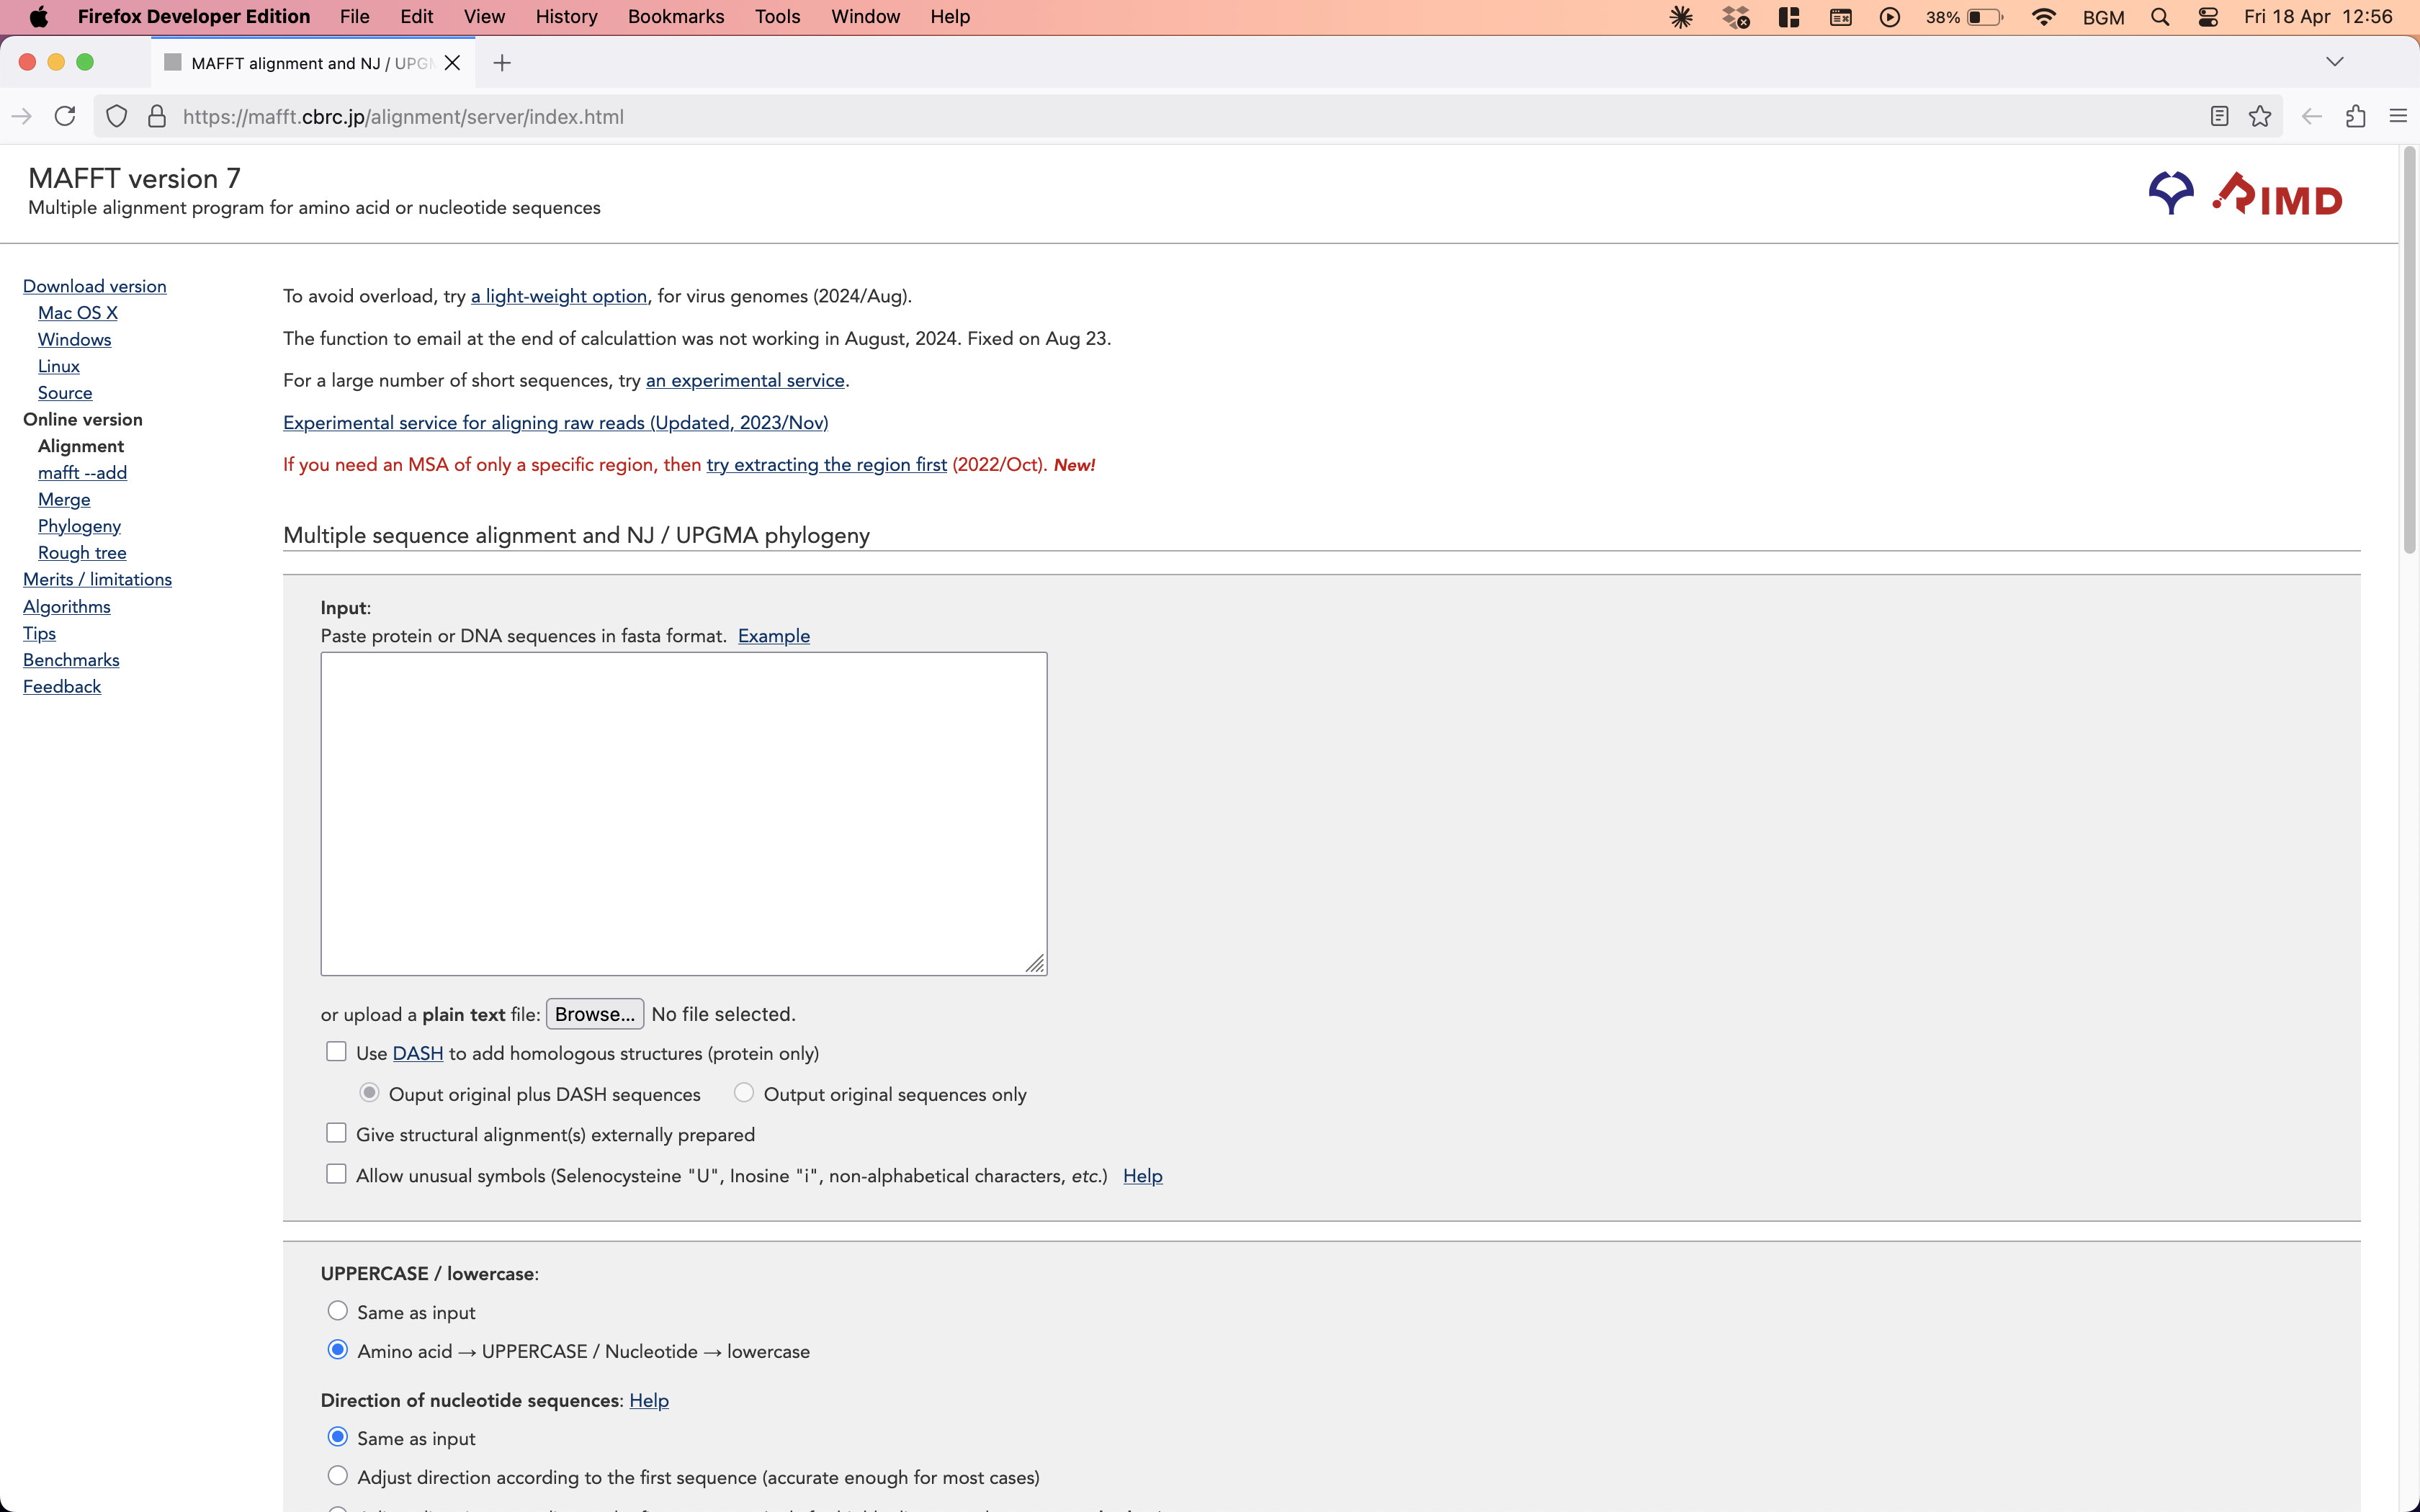
\includegraphics[width=0.7\textwidth]{img/mafft.png}
	\end{figure}
\end{document}